\documentclass{article}
\usepackage[margin=1in]{geometry}
\usepackage{amsmath,amsthm,amssymb}
\usepackage{bbm,enumerate,mathtools}
\usepackage{tikz,pgfplots}
\usepackage{chessboard}
\usepackage[hidelinks]{hyperref}
\usepackage{multicol} % Problem 35

\newenvironment{question}{\begin{trivlist}\item[\textbf{Question.}]}{\end{trivlist}}
\newenvironment{note}{\begin{trivlist}\item[\textbf{Note.}]}{\end{trivlist}}
\newenvironment{references}{\begin{trivlist}\item[\textbf{References.}]}{\end{trivlist}}
\newenvironment{related}{\begin{trivlist}\item[\textbf{Related.}]\end{trivlist}\begin{enumerate}}{\end{enumerate}}


\begin{document}
\rating{2}{2}
Starting with an $n \times m$ grid, remove one corner at a time (uniformly at
random) until the grid is gone.
\begin{figure}[!h]
  \centering
  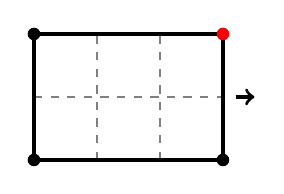
\begin{tikzpicture}[scale=0.8]
    \draw[dashed, gray] (0,0) grid (3,2);
    \draw[very thick] (0,0) rectangle (3,2);
    \fill[red] (3,2) circle (0.1cm);
    \foreach \x/\y in {0/0, 0/2, 3/0} {\fill (\x,\y) circle (0.1cm);}
    \draw[very thick, ->] (3.2,1)--(3.5,1);
  \end{tikzpicture}
  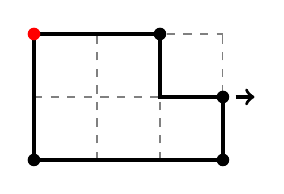
\begin{tikzpicture}[scale=0.8]
    \draw[dashed, gray] (0,0) grid (3,2);
    \draw[very thick] (0,0)--(0,2)--(2,2)--(2,1)--(3,1)--(3,0)--cycle;
    \fill[red] (0,2) circle (0.1cm);
    \foreach \x/\y in {0/0, 2/2, 3/0, 3/1} {\fill (\x,\y) circle (0.1cm);}
    \draw[very thick, ->] (3.2,1)--(3.5,1);
  \end{tikzpicture}
  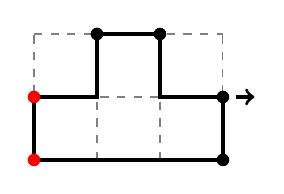
\begin{tikzpicture}[scale=0.8]
    \draw[dashed, gray] (0,0) grid (3,2);
    \draw[very thick] (0,0)--(0,1)--(1,1)--(1,2)--(2,2)--(2,1)--(3,1)--(3,0)--cycle;
    \fill[red] (0,0) circle (0.1cm); \fill[red] (0,1) circle (0.1cm);
    \foreach \x/\y in {1/2, 2/2, 3/0, 3/1} {\fill (\x,\y) circle (0.1cm);}
    \draw[very thick, ->] (3.2,1)--(3.5,1);
  \end{tikzpicture}
  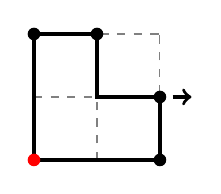
\begin{tikzpicture}[scale=0.8]
    \draw[dashed, gray] (0,0) grid (2,2);
    \draw[very thick] (0,0)--(0,2)--(1,2)--(1,1)--(2,1)--(2,0)--cycle;
    \fill[red] (0,0) circle (0.1cm);
    \foreach \x/\y in {0/2, 1/2, 2/0, 2/1} {\fill (\x,\y) circle (0.1cm);}
    \draw[very thick, ->] (2.2,1)--(2.5,1);
  \end{tikzpicture}
  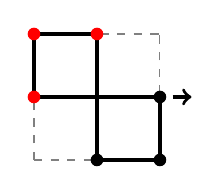
\begin{tikzpicture}[scale=0.8]
    \draw[dashed, gray] (0,0) grid (2,2);
    \draw[very thick] (1,0)--(1,1)--(0,1)--(0,2)--(1,2)--(1,1)--(2,1)--(2,0)--cycle;
    \fill[red] (0,1) circle (0.1cm); \fill[red] (0,2) circle (0.1cm); \fill[red] (1,2) circle (0.1cm);
    \foreach \x/\y in {1/0, 2/0, 2/1} {\fill (\x,\y) circle (0.1cm);}
    \draw[very thick, ->] (2.2,1)--(2.5,1);
  \end{tikzpicture}
  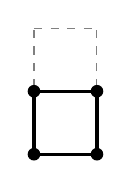
\begin{tikzpicture}[scale=0.8]
    \draw[dashed, gray] (0,0) grid (1,2);
    \draw[very thick] (0,0) rectangle (1,1);
    \foreach \x/\y in {0/0, 0/1, 1/0, 1/1} {\fill (\x,\y) circle (0.1cm);}
  \end{tikzpicture}

  \caption{
    An example of a process starting with a $2 \times 3$ grid.
  }
\end{figure}

\begin{question}
  If a stopping point is chosen randomly, how many corners are expected?
\end{question}
\begin{related}
  \item What if the deletion is uniform with respect to faces instead of
    vertices?
  \item How many sides are expected?
  \item If all polygons in the process are considered, what is the expected
    number of corners on the polygon with the greatest number of corners?
  \item What figure produces the greatest number of corners?
  \item How many possible processes exist (up to, say, dihedral action)?
  \item What if each figure must stay path connected?
  \item What if paths cannot travel through corners? (e.g. the second-to-last
    figure is illegal.)
\end{related}

\end{document}
